\documentclass[12pt,a4paper]{article}
% !TEX root = paper.tex
% ── Packages ─────────────────────────────────────────────────────────────────
\usepackage[utf8]{inputenc}
\usepackage[T1]{fontenc}
\usepackage{lmodern}
\usepackage[margin=2.5cm]{geometry}
\usepackage{amsmath,amssymb}
\usepackage{booktabs}
\usepackage{multirow}
\usepackage{array}
\usepackage{longtable}
\usepackage{graphicx}
\usepackage{float}
\usepackage{caption}
\usepackage{subcaption}
\usepackage{hyperref}
\usepackage{xcolor}
\usepackage{setspace}
\usepackage[numbers]{natbib}
\usepackage{microtype}
\usepackage{parskip}
\usepackage{enumitem}
\usepackage{siunitx}

% ── Hyperref setup ────────────────────────────────────────────────────────────
\hypersetup{
  colorlinks=true,
  linkcolor=blue!70!black,
  citecolor=green!50!black,
  urlcolor=blue!70!black,
}

% ── Custom commands ───────────────────────────────────────────────────────────
\newcommand{\pval}[1]{$p = #1$}
\newcommand{\rval}[1]{$r = #1$}
\newcommand{\chisq}[1]{$\chi^2 = #1$}
\newcommand{\rmse}[1]{\text{RMSE} = #1\,\text{kt}}
\newcommand{\Hstat}[1]{$H = #1$}
\newcommand{\Fstat}[1]{$F = #1$}
\newcommand{\etasq}[1]{$\eta^2 = #1$}
\newcommand{\CrV}[1]{$V = #1$}
\newcommand{\rbs}[1]{$r_{\text{rb}} = #1$}

\definecolor{notecolor}{RGB}{80,80,160}
\newcommand{\caution}[1]{\textcolor{notecolor}{\textit{#1}}}

% ─────────────────────────────────────────────────────────────────────────────
\begin{document}

\begin{titlepage}
  \centering
  \vspace*{2cm}
  {\LARGE\bfseries Vedic Astrology and Astronomical Features\\[6pt]
   in Tropical Cyclone Intensity Modelling:\\[4pt]
   A Large-Scale Empirical Assessment\par}
  \vspace{1.5cm}
  {\large Hariramanan Sivakumar \par}
  \vspace{0.5cm}
  {\normalsize \textit{Independent Research}\par}
  \vspace{1cm}
  {\normalsize\texttt{reachariramanan@gmail.com}\par}
  \vfill
  {\normalsize May 2026\par}
  \vspace{1.5cm}
  \rule{\linewidth}{0.4pt}
  \vspace{0.3cm}
  \begin{abstract}
    \noindent
    We present the first large-scale empirical investigation of whether Vedic
    Panchang (Hindu calendar) categories and planetary astronomical positions
    carry detectable signal for tropical cyclone intensity.
    Using 47{,}533 track observations from 944 global storms spanning
    2016--2026, we construct a 222-feature dataset encompassing 14
    meteorological, 18 Panchangam, and 190 scientific-astronomical predictors,
    and evaluate predictive performance through multiple complementary methods:
    chronological holdout regression, five-fold forward-chaining cross-validation,
    permutation group importance, non-parametric hypothesis testing with effect
    size quantification, and confound-adjusted stratified analysis.
    Our primary finding is a \textbf{null result}: adding Vedic features to a
    meteorological baseline degrades wind-change root-mean-square error (RMSE)
    by 14.3\% and the full model fails to outperform the meteorological baseline
    in 4 of 5 temporal folds.
    Two secondary signals survive Bonferroni correction but carry negligible
    practical effect sizes: a lunar-phase association with rapid intensification
    (RI; $\chi^2 = 19.66$, $p = 0.006$, Cram\'er's $V \approx 0.020$) and a
    consistent negative correlation between planetary speed and storm bearing
    direction ($\rho \approx -0.18$, $r^2 \approx 3\%$).
    We document that statistical significance is inflated by dataset scale
    ($N \approx 47{,}533$) and identify seasonal confounding as the primary driver
    of apparent Vedic categorical effects.
    These findings provide a methodological template for rigorous evaluation of
    non-conventional features in meteorological machine learning.
  \end{abstract}
\end{titlepage}

\tableofcontents
\clearpage

% =============================================================================
\section{Introduction}
\label{sec:intro}
% =============================================================================

Tropical cyclones pose severe societal risks, and improving the accuracy of
intensity forecasts remains an active area of meteorological research
\citep{emanuel2003tropical}.
Alongside conventional numerical weather prediction and machine learning
approaches that exploit atmospheric and oceanic variables, there exists a
long-standing traditional claim, rooted in Vedic astrology, that planetary
positions and Hindu calendar cycles modulate weather events and natural
disasters.
Vedic astrology encodes the positions of the Sun, Moon, and seven classical
planets into a rich system of named categories: \textit{Tithi} (lunar day),
\textit{Nakshatra} (lunar mansion), \textit{Yoga} (Sun--Moon arc interval),
\textit{Karana} (half-Tithi), and several dozen more.
These categories are deterministic functions of planetary ephemerides and are
therefore computable for any date, time, and location.

This determinism makes Vedic features unusual among non-conventional predictors:
they are neither noisy survey data nor domain-expert judgements but precise
mathematical transformations of astronomical coordinates.
If any Vedic category were genuinely associated with cyclone intensity, it would
imply that the underlying astronomical geometry carries information about storm
dynamics beyond what standard meteorological variables encode.

To our knowledge, no prior study has subjected these claims to a rigorous
large-scale test against a diverse global cyclone database.
We address this gap by assembling data from 944 storms across all major ocean
basins, pairing track observations with Vedic Panchang values computed using the
Drik Panchang astronomy engine, and conducting a battery of tests whose design
explicitly addresses the statistical pathologies common in large-$N$ astronomical
association studies.

\subsection*{Research Questions}

\begin{enumerate}[label=\textbf{RQ\arabic*.}]
  \item Do Vedic Panchang features improve next-step storm intensity prediction
        over a meteorological baseline?
  \item Is there a statistically and practically significant association between
        lunar phase and rapid intensification?
  \item Do planetary speeds correlate with storm track bearing beyond chance?
  \item Do planets in apparent retrograde motion correspond to measurably
        different storm intensity distributions?
  \item Do Vedic categorical wind associations persist after removing the
        dominant seasonal--geographic confound?
\end{enumerate}

\subsection*{Summary of Contributions}

\begin{itemize}
  \item First large-scale ($N = 47{,}533$ observations) empirical test of Vedic
        astrology features in tropical cyclone forecasting.
  \item Comprehensive effect size analysis distinguishing statistical from
        practical significance across all findings.
  \item A confound-adjusted partial Kruskal--Wallis framework for testing
        categorical astronomical associations within season$\times$basin strata.
  \item A novel lunar-phase$\times$lifecycle interaction analysis showing that
        RI associations with lunar phase are lifecycle-stage dependent.
  \item Open release of the 222-feature parsed dataset and all analysis scripts.
\end{itemize}

% =============================================================================
\section{Data and Features}
\label{sec:data}
% =============================================================================

\subsection{Storm Track Data}

We use best-track data assembled from multiple regional operational meteorological
agencies for 944 tropical cyclones active between July 2016 and January 2026,
spanning the North Atlantic, Western Pacific, North Indian Ocean, South Indian
Ocean, and South Pacific basins.
Each track observation records the storm centre position (latitude, longitude),
maximum sustained wind speed (knots), minimum central pressure (hPa), and UTC
timestamp.
Track observations are provided at variable intervals (predominantly 3--6 h),
yielding 47{,}533 observations in total after filtering incomplete records.

\subsection{Vedic Panchang Features}

For each track observation, Vedic Panchang attributes were computed using the
Drik Panchang astronomy engine at the storm centre location and local time.
This produces 18 categorical and derived features (Table~\ref{tab:panchang_features}),
including the five canonical Panchang limbs plus additional calendar and celestial
quantities.
Continuous Vedic planetary parameters (sidereal degree, speed in degrees per day,
right ascension, declination, and Nakshatra pada) were computed for 15 bodies:
Sun, Moon, Mars, Mercury, Jupiter, Venus, Saturn, Uranus, Neptune, Rahu (north
lunar node), Ketu (south lunar node), Yama, Arun, Varun, and Spashtha Rahu/Ketu,
yielding 75 numeric Vedic features.

\begin{table}[H]
  \centering
  \caption{Vedic Panchang categorical features used in this study.}
  \label{tab:panchang_features}
  \small
  \begin{tabular}{llp{7cm}}
    \toprule
    \textbf{Feature} & \textbf{Type} & \textbf{Description} \\
    \midrule
    Tithi       & Categorical (30)  & Lunar day (Sun--Moon elongation in $12^\circ$ steps) \\
    Nakshatra   & Categorical (27)  & Lunar mansion (Moon's sidereal position in $13.3^\circ$ segments) \\
    Yoga        & Categorical (27)  & Sun+Moon sidereal longitude mod $360^\circ$, divided into 27 equal parts \\
    Karana      & Categorical (11)  & Half-Tithi period \\
    Paksha      & Binary            & Waxing (\textit{Shukla}) or waning (\textit{Krishna}) lunar fortnight \\
    Moonsign    & Categorical (12)  & Sidereal zodiac sign of the Moon \\
    Sunsign     & Categorical (12)  & Sidereal zodiac sign of the Sun \\
    Drik Ritu   & Categorical (6)   & Observational season (equinox/solstice based) \\
    Vedic Ritu  & Categorical (6)   & Traditional Hindu season \\
    Drik Ayana  & Binary            & Northern/southern hemisphere Sun path \\
    Vedic Ayana & Binary            & Traditional equivalent of Ayana \\
    Anandadi Yoga & Categorical (9) & Auspiciousness index derived from weekday+Nakshatra \\
    Tamil Yoga  & Categorical (5)   & Tamil calendar auspiciousness classification \\
    Samvatsara  & Categorical (60)  & 60-year Jupiter cycle year name \\
    Rahu Kalam  & Time range        & Daily inauspicious period (time-range string) \\
    Yamaganda   & Time range        & Secondary inauspicious period \\
    Gulikai Kalam & Time range      & Tertiary inauspicious period \\
    Weekday     & Categorical (7)   & Hindu weekday \\
    \bottomrule
  \end{tabular}
\end{table}

\subsection{Astronomical Features (Skyfield)}

Skyfield ephemeris computations at each storm position and timestamp provide 90
numeric features covering altitude, azimuth, right ascension, declination,
ecliptic longitude and latitude, and derived trigonometric transforms
($\sin/\cos$ of altitude and azimuth) for the Sun, Moon, and seven classical
planets.

\subsection{Meteorological Features}

Fourteen standard meteorological and derived kinematic features are used as the
baseline: wind speed (kt), pressure (hPa), latitude, longitude, hour (UTC),
day of year, day of week, month, movement speed, displacement, and four
spline-fitted track geometry features (curvature, bearing, displacement,
length in degrees).

\caution{Leakage note: the spline features encode the smoothed forecast track
geometry and may carry implicit information about future storm position.
Correlations involving these features should be interpreted with caution.}

\subsection{Target Variable}

The primary regression target is the \textit{next-step wind delta}
($\Delta w_{t+1} = w_{t+1} - w_t$), constructed by shifting the wind column
one step forward within each storm group.
For classification experiments, rapid intensification (RI) is defined as
$\Delta w \geq 10\,\text{kt}$ per step (Section~\ref{sec:models}), following
the adaptive threshold logic of script 07.
The 24-hour RI threshold of $\geq 30\,\text{kt}$ used in hypothesis H2
(Section~\ref{sec:h2}) follows a rolling-window definition distinct from
the step-wise target and the two should not be directly compared.

\subsection{Dataset Summary}

\begin{table}[H]
  \centering
  \caption{Dataset summary statistics.}
  \label{tab:dataset}
  \begin{tabular}{lr}
    \toprule
    \textbf{Property} & \textbf{Value} \\
    \midrule
    Total track observations            & 47{,}533 \\
    Unique storms                       & 944 \\
    Date range                          & 2016-07-15 -- 2026-01-24 \\
    Ocean basins                        & 7 \\
    Mean wind speed                     & 49.9 kt \\
    Median wind speed                   & 40.0 kt \\
    Wind skewness                       & 1.35 (right-skewed) \\
    Pressure range                      & 882--1019 hPa \\
    Meteorological features             & 14 \\
    Panchangam features                 & 18 \\
    Scientific/astronomical features    & 190 \\
    Total features                      & 222 \\
    Missing: spline features            & 15.4\% \\
    Missing: cone features              & $\approx$99\% (excluded) \\
    \bottomrule
  \end{tabular}
\end{table}

% =============================================================================
\section{Methods}
\label{sec:methods}
% =============================================================================

\subsection{Predictive Modelling}
\label{sec:models}

We train Random Forest regressors (200 trees, max depth 18, min samples per
leaf 2) in four block configurations:
\begin{enumerate}
  \item \textbf{Meteo only}: 14 meteorological features.
  \item \textbf{Meteo + Panchang}: 14 meteorological + 18 Panchangam features.
  \item \textbf{Full}: all 222 features.
  \item \textbf{Stacked residual}: a meteorological stage-A model whose residuals
        are fed to a stage-B model on Panchang + scientific features.
\end{enumerate}
All categorical features are ordinal-label-encoded from the training split only
(test categories unseen during training are mapped to $-1$).
Missing numeric values are imputed with the training-set median per column.

\paragraph{Train--test split.} A chronological 80/20 split is applied at the
individual observation level: observations before 2023-10-21 form the training
set ($n = 37{,}274$) and subsequent observations form the held-out test set
($n = 9{,}315$).

\paragraph{Forward-chaining cross-validation.} Five temporal folds are defined
at chronological quantiles (0.2, 0.4, 0.6, 0.7, 0.9).
Each fold uses all data before the boundary for training, and a 120-day window
after the boundary for validation, requiring $\geq 5{,}000$ training and
$\geq 500$ validation observations.
This prevents within-storm data leakage from standard $k$-fold approaches.

\paragraph{Group permutation importance.} The contribution of each feature group
(meteo, Panchang, scientific) to the full model is estimated by permuting all
features in that group simultaneously ($n_\text{repeats} = 5$) and recording
the mean RMSE lift.

\paragraph{Classification.} An adaptive RI threshold selects the strictest
threshold in $\{20, 15, 10, 5\}$~kt/step that yields $\geq 100$ positive
training cases and $\geq 20$ positive test cases.
For the present dataset this resolves to 10~kt/step (3{,}053 training and 1{,}024
test positives).

\subsection{Hypothesis Testing}
\label{sec:hyp_methods}

\paragraph{Non-parametric rationale.} Shapiro--Wilk tests confirm that all
key variables are non-normal ($p < 10^{-30}$ for wind, pressure, latitude,
longitude; wind skewness = 1.35).
We therefore use non-parametric tests throughout: Mann--Whitney $U$ for
two-group comparisons, Kruskal--Wallis for $k$-group comparisons, and
Spearman $\rho$ for monotone associations.

\paragraph{Multiple comparison correction.} Where multiple tests are conducted
within a family, Benjamini--Hochberg false discovery rate (BH-FDR) correction
is applied.
Across the seven primary hypothesis groups, a Bonferroni-corrected threshold
of $\alpha/7 \approx 0.0071$ is used.

\paragraph{Effect sizes.} Given $N \approx 47{,}533$, even trivially small
effects produce highly significant $p$-values.
We therefore accompany every significant result with an appropriate effect size
measure:
\begin{itemize}
  \item \textbf{Rank-biserial $r$} for Mann--Whitney results:
        $r_\text{rb} = 1 - 2U/(n_1 n_2)$.
        Thresholds: small $< 0.10$, medium $0.10$--$0.30$, large $> 0.30$.
  \item \textbf{Cohen's $d$} (pooled SD) for two-group comparisons.
        Thresholds: small $< 0.20$, medium $0.20$--$0.50$, large $> 0.50$.
  \item \textbf{Epsilon-squared} ($\varepsilon^2 = (H - k + 1)/(N - k)$)
        for Kruskal--Wallis.
  \item \textbf{Cram\'er's $V$} for chi-squared tests:
        $V = \sqrt{\chi^2 / (N \cdot (\min(r,c)-1))}$.
        Thresholds: small $< 0.10$, medium $0.10$--$0.30$, large $> 0.30$.
  \item \textbf{Eta-squared} ($\eta^2 = F \cdot \text{df}_b / (F \cdot \text{df}_b + \text{df}_w)$)
        for ANOVA.
  \item \textbf{$r^2$ (Spearman)} for monotone correlations.
\end{itemize}

\paragraph{H1 -- Vedic predictive power.}
Trained with a chronological split, the Vedic and meteo+Vedic models are
compared to the meteo-only baseline by RMSE (lower is better).
A positive percentage RMSE change indicates degradation.

\paragraph{H2 -- Lunar phase and rapid intensification.}
The 24-hour RI indicator ($\Delta w_\text{24h} \geq 30\,\text{kt}$ via
per-storm rolling window) is cross-tabulated against 8 equal lunar-phase bins
($45^\circ$ each, anchored at the Moon--Sun ecliptic angle) and tested with a
chi-squared test.
To further decompose the signal, we repeat the test within each lifecycle phase
(Genesis, Intensify, Mature, Dissipate), derived as described in H5.

\paragraph{H3 -- Planetary speed and trajectory.}
Spearman $\rho$ is computed between each Vedic planetary speed
(deg\,day$^{-1}$) and \texttt{spline\_bearing\_deg} for all 60 speed--target
pairs.
Monotonicity is verified by binning each speed feature into quintiles and
computing the Spearman rank correlation of quintile index versus median bearing.

\paragraph{H4 -- Retrograde effects.}
Each planet is classified as retrograde when its speed $< 0$.
Mann--Whitney $U$ tests compare the wind distributions of retrograde versus
direct observations with BH-FDR correction.

\paragraph{H5 -- Confound-adjusted Vedic categorical analysis.}
Each observation is assigned to a stratum defined as
\texttt{drik\_ritu} $\times$ \texttt{basin\_geo}.
Within each stratum having $\geq 100$ observations, Kruskal--Wallis tests are
run for Tithi, Nakshatra, Yoga, and Moonsign, requiring $\geq 3$ categories
with $\geq 10$ observations each.
BH-FDR correction is applied across all $p$-values within each variable.
The percentage of strata showing significant within-stratum KW signal is
reported.

\subsection{Lifecycle Phase Classification}

Storm lifecycle is partitioned into four phases using normalised track
progress $\tau = (k - k_{\min}) / \max(k_{\max} - k_{\min}, 1)$, where $k$ is
track index within each storm:
Genesis ($\tau \in [0, 0.2]$), Intensification ($\tau \in (0.2, 0.5]$),
Mature ($\tau \in (0.5, 0.7]$), Dissipation ($\tau \in (0.7, 1.0]$).
This approximation assumes a monotonic single-peak intensification curve;
storms that re-intensify after weakening may be mislabelled in later phases.

% =============================================================================
\section{Results}
\label{sec:results}
% =============================================================================

\subsection{RQ1: Predictive Modelling}
\label{sec:rq1}

Table~\ref{tab:rmse} presents RMSE and MAE on the chronological test set.
The meteorological-only model achieves the best performance ($\rmse{4.164}$),
and every addition of Vedic or astronomical features strictly increases error.
Adding Panchang features alone degrades RMSE by 4.9\% ($4.164 \to 4.372$~kt)
and the full model degrades it by 8.4\% ($4.164 \to 4.515$~kt).

\begin{table}[H]
  \centering
  \caption{Regression performance on the chronological holdout test set
           ($n = 9{,}315$). Lower RMSE and MAE are better.
           $\Delta$RMSE\% is computed relative to the \textit{Meteo only} baseline.}
  \label{tab:rmse}
  \begin{tabular}{lrrr}
    \toprule
    \textbf{Model} & \textbf{RMSE (kt)} & \textbf{MAE (kt)} & \boldmath$\Delta$\textbf{RMSE\%} \\
    \midrule
    Meteo only            & 4.164 & 2.540 & --- \\
    Stacked residual      & 4.192 & 2.582 & $+0.7\%$ \\
    Meteo + Panchang      & 4.372 & 2.685 & $+4.9\%$ \\
    Full (all blocks)     & 4.515 & 2.921 & $+8.4\%$ \\
    \bottomrule
  \end{tabular}
\end{table}

Forward-chaining cross-validation (Table~\ref{tab:cv}) confirms this pattern
across time: the meteorological model wins or ties in 4 of 5 folds, with the
full model consistently worse in folds 2--5 by 0.15--0.48~kt.

\begin{table}[H]
  \centering
  \caption{Forward-chaining cross-validation RMSE (kt) by fold and model.
           Fold boundaries represent chronological quantiles of the training set.
           Bold indicates the best-performing model in each fold.}
  \label{tab:cv}
  \begin{tabular}{lrrrr}
    \toprule
    \textbf{Fold} & \textbf{Boundary} & \textbf{Meteo only} & \textbf{Full} & \textbf{Stacked} \\
    \midrule
    1 & 2018-08-06 & \textbf{3.369} & 3.357 & 3.373 \\
    2 & 2020-01-23 & \textbf{3.753} & 3.885 & 3.813 \\
    3 & 2021-09-13 & \textbf{3.191} & 3.508 & 3.188 \\
    4 & 2023-04-22 & \textbf{3.209} & 3.685 & 3.211 \\
    5 & 2025-01-31 & \textbf{3.797} & 4.090 & 3.875 \\
    \bottomrule
    \multicolumn{2}{l}{\textit{Mean}} & \textbf{3.464} & 3.705 & 3.492 \\
    \bottomrule
  \end{tabular}
\end{table}

Group permutation importance (Table~\ref{tab:group_imp}) confirms that the
meteorological group dominates: permuting all 14 meteo features raises RMSE by
$+0.582\pm0.032$~kt, while permuting all 18 Panchang features raises it by only
$+0.010\pm0.005$~kt — less than 2\% of the meteo contribution.

\begin{table}[H]
  \centering
  \caption{Group-level permutation RMSE lift on the full model test set
           ($n_\text{repeats} = 5$). Higher lift indicates greater contribution.}
  \label{tab:group_imp}
  \begin{tabular}{lrr}
    \toprule
    \textbf{Group} & \textbf{Mean RMSE lift (kt)} & \textbf{SD} \\
    \midrule
    Meteorological      & 0.582 & 0.032 \\
    Scientific/Astro    & 0.175 & 0.005 \\
    Vedic/Panchang      & 0.010 & 0.005 \\
    \bottomrule
  \end{tabular}
\end{table}

For RI classification (threshold $\geq 10$~kt/step), the meteo-only model
achieves AUC-ROC = 0.707 while the full model degrades to AUC-ROC = 0.429 —
below chance — demonstrating that adding 190 astronomical features actively
harms RI classification.
Both models produce $F_1 = 0.0$ at threshold 0.5, indicating that RI events
remain difficult to classify with the available features regardless of the
feature set.

\subsection{RQ2: Lunar Phase and Rapid Intensification}
\label{sec:h2}

A chi-squared test of the 24-hour RI indicator ($\Delta w_\text{24h} \geq 30$~kt,
rolling window) against 8 lunar-phase bins yields
$\chi^2 = 19.66$, $p = 0.006$, $\mathrm{dof} = 7$,
which survives the Bonferroni-corrected threshold of $\alpha/7 \approx 0.0071$.
However, Cram\'er's $V = \sqrt{19.66/47{,}533} \approx 0.020$ places this firmly
in the ``small'' range.

Table~\ref{tab:ri_lunar} shows RI rates per lunar phase.
The Waning Crescent phase has the highest absolute RI count (83 events, RI rate
1.33\%) and Waxing Crescent the lowest (49 events, RI rate 0.79\%) — a 37\%
relative range.

\begin{table}[H]
  \centering
  \caption{Rapid intensification (RI) rate by lunar phase.
           RI defined as $\Delta w_\text{24h} \geq 30$~kt (rolling window).
           Waning Crescent is highlighted as the peak RI phase.}
  \label{tab:ri_lunar}
  \begin{tabular}{lrrr}
    \toprule
    \textbf{Lunar Phase} & \textbf{RI Events} & \textbf{Total Obs} & \textbf{RI Rate} \\
    \midrule
    New Moon              &  80 & 6{,}529 & 1.23\% \\
    Waxing Crescent       &  49 & 6{,}188 & 0.79\% \\
    First Quarter         &  82 & 6{,}024 & 1.36\% \\
    Waxing Gibbous        &  79 & 5{,}419 & 1.46\% \\
    Full Moon             &  65 & 5{,}360 & 1.21\% \\
    Waning Gibbous        &  81 & 5{,}649 & 1.43\% \\
    Third Quarter         &  64 & 6{,}115 & 1.05\% \\
    \textbf{Waning Crescent} & \textbf{83} & \textbf{6{,}249} & \textbf{1.33\%} \\
    \bottomrule
  \end{tabular}
\end{table}

\paragraph{Lifecycle interaction.}
When the chi-squared test is repeated within each lifecycle phase separately
(Table~\ref{tab:ri_lifecycle}), the lunar-phase RI signal is significant in
the Genesis ($p = 0.0008$) and Dissipation ($p = 0.001$) stages but
not in the Mature phase ($p = 0.265$).
This indicates that the aggregate signal is not uniformly distributed across
the storm lifetime: forming and decaying storms show stronger lunar-phase
modulation of RI rate than storms at peak intensity.

\begin{table}[H]
  \centering
  \caption{Chi-squared test for lunar-phase distribution of RI events
           within each storm lifecycle phase.}
  \label{tab:ri_lifecycle}
  \begin{tabular}{lrrr}
    \toprule
    \textbf{Lifecycle Phase} & \boldmath$\chi^2$ & \boldmath$p$ & \textbf{N obs} \\
    \midrule
    Genesis       & 24.88 & 0.0008 & 9{,}870 \\
    Intensify     & 15.99 & 0.025  & 14{,}285 \\
    Mature        &  8.83 & 0.265  & 9{,}011 \\
    Dissipate     & 24.38 & 0.001  & 14{,}367 \\
    \bottomrule
  \end{tabular}
\end{table}

\subsection{RQ3: Planetary Speed and Storm Bearing}
\label{sec:h3}

Table~\ref{tab:h3_spearman} presents Spearman $\rho$ between Vedic planetary
speeds and \texttt{spline\_bearing\_deg}.
Four planets (Yama, Shani, Varun, Surya) show nominally medium-strength
correlations ($|\rho| > 0.10$) that are overwhelmingly significant in $p$-value
terms but explain only 2.5--3.2\% of bearing variance ($r^2 \leq 0.032$).

\begin{table}[H]
  \centering
  \caption{Top-10 Spearman correlations between Vedic planetary speed
           (deg\,day$^{-1}$) and storm bearing (deg), sorted by $|\rho|$.
           All $p < 10^{-20}$. $r^2$ = $\rho^2$ (variance explained).}
  \label{tab:h3_spearman}
  \begin{tabular}{lrrr}
    \toprule
    \textbf{Speed Feature} & \boldmath$\rho$ & \boldmath$p$ & \boldmath$r^2$ \\
    \midrule
    Yama (vedic\_yam\_speed)    & $-0.178$ & $3.8\times10^{-271}$ & 0.032 \\
    Shani (Saturn)              & $-0.168$ & $2.2\times10^{-241}$ & 0.028 \\
    Varun (Neptune)             & $-0.167$ & $1.0\times10^{-236}$ & 0.028 \\
    Surya (Sun)                 & $-0.158$ & $6.2\times10^{-213}$ & 0.025 \\
    Guru (Jupiter)              & $-0.056$ & $8.6\times10^{-28}$  & 0.003 \\
    Arun (Uranus)               & $-0.049$ & $1.1\times10^{-21}$  & 0.002 \\
    Mangal (Mars)               & $-0.043$ & $2.7\times10^{-17}$  & 0.002 \\
    Spashtha Rahu               & $+0.035$ & $4.9\times10^{-12}$  & 0.001 \\
    Spashtha Ketu               & $+0.035$ & $4.9\times10^{-12}$  & 0.001 \\
    Budha (Mercury)             & $+0.028$ & $3.8\times10^{-8}$   & 0.001 \\
    \bottomrule
  \end{tabular}
\end{table}

Quintile dose-response analysis confirms that all significant correlations are
\emph{perfectly monotone} (Spearman $\rho_\text{quintile} = -1.0$ for all
tested speed features): as planetary speed increases from its lowest quintile
(Q1) to its highest (Q5), median storm bearing decreases monotonically from
$\approx 279^\circ$ to $\approx 217^\circ$.
This gradient ($\approx 62^\circ$ range across quintiles) is consistent across all
three tested planets (Yama, Shani, Surya), suggesting a systematic relationship
rather than an outlier-driven artefact.
Nevertheless, the $r^2 \leq 3.2\%$ limits operational utility.

\caution{Spline leakage caution:} \texttt{spline\_bearing\_deg} encodes the
smoothed forecast track bearing and may carry implicit future trajectory
information.
We cannot rule out that the planetary speed correlations partly reflect this
latent future information rather than a direct astronomical--dynamical coupling.

\subsection{RQ4: Retrograde Planet Effects on Wind Intensity}
\label{sec:h4}

Table~\ref{tab:retrograde} summarises the Mann--Whitney $U$ tests comparing
wind distributions between retrograde and direct planetary phases.
All seven planets yield statistically significant differences, but every
rank-biserial correlation is below the small-effect threshold of $|r_\text{rb}| < 0.10$.

\begin{table}[H]
  \centering
  \caption{Retrograde vs.\ direct wind intensity comparison (Mann--Whitney $U$).
           $r_\text{rb}$ = rank-biserial correlation; $d$ = Cohen's $d$.
           All effects classified as \emph{small}.}
  \label{tab:retrograde}
  \begin{tabular}{lrrrrrrr}
    \toprule
    \textbf{Planet} & \textbf{Retro \%} & \textbf{Retro med.} & \textbf{Direct med.} &
    \textbf{Diff (kt)} & \boldmath$p$ & \boldmath$r_\text{rb}$ & \boldmath$d$ \\
    \midrule
    Guru (Jupiter) & 29.7 & 40 & 42 & $-2$ & $2.3\times10^{-23}$ & $+0.058$ & $-0.117$ \\
    Shani (Saturn) & 46.3 & 40 & 40 & $0$  & $5.0\times10^{-6}$  & $-0.024$ & $+0.013$ \\
    Mangal (Mars)  &  9.1 & 41 & 40 & $+1$ & $4.5\times10^{-4}$  & $-0.032$ & $+0.040$ \\
    Budha (Mercury)& 20.8 & 40 & 40 & $0$  & $2.3\times10^{-22}$ & $+0.063$ & $-0.102$ \\
    Shukra (Venus) &  7.9 & 45 & 40 & $+5$ & $6.6\times10^{-6}$  & $-0.044$ & $+0.075$ \\
    Arun (Uranus)  & 51.8 & 43 & 40 & $+3$ & $1.0\times10^{-38}$ & $-0.069$ & $+0.125$ \\
    Varun (Neptune)& 60.3 & 43 & 39 & $+4$ & $2.3\times10^{-59}$ & $-0.088$ & $+0.139$ \\
    \bottomrule
  \end{tabular}
\end{table}

Three observations are noteworthy.
First, Varun (Neptune) and Arun (Uranus) are retrograde for 60\% and 52\% of
all observations respectively — their retrograde phase is simply the
majority condition during long spans of the dataset and does not represent
a meaningfully rare astronomical event.
Second, even Shukra (Venus, retrograde only 7.9\% of observations) shows a
median wind difference of only 5~kt with $|r_\text{rb}| = 0.044$ (small).
Third, the Cohen's $d$ values ($d \leq 0.14$) are uniformly below the small
threshold for all seven planets, confirming the effect size assessment.

\subsection{RQ5: Confound-Adjusted Vedic Categorical Analysis}
\label{sec:h5}

Table~\ref{tab:kw_global} shows global Kruskal--Wallis results for Vedic
categorical variables against wind speed.
The two strongest signals — Drik Ritu ($H = 1{,}214$) and Sunsign ($H = 1{,}123$)
— are deterministic functions of the solar calendar and serve as seasonal proxies
rather than independent Vedic variables.

\begin{table}[H]
  \centering
  \caption{Global Kruskal--Wallis statistics for Vedic categorical variables
           against wind speed ($N = 47{,}533$). $\varepsilon^2$ = epsilon-squared
           (effect size). All listed results survive BH-FDR correction.}
  \label{tab:kw_global}
  \begin{tabular}{lrrrrl}
    \toprule
    \textbf{Variable} & \boldmath$H$ & \boldmath$p$ & \boldmath$k$ &
    \boldmath$\varepsilon^2$ & \textbf{Note} \\
    \midrule
    Drik Ritu    & 1{,}214 & $2.7\times10^{-260}$ & 6  & 0.025 & Seasonal proxy \\
    Sunsign      & 1{,}123 & $5.9\times10^{-234}$ & 12 & 0.020 & Solar calendar proxy \\
    Yoga         &   143   & $3.4\times10^{-18}$  & 27 & ---   & Confound check below \\
    Nakshatra    &   116   & $2.4\times10^{-13}$  & 27 & ---   & Confound check below \\
    Drik Ayana   &   103   & $4.0\times10^{-24}$  & 2  & ---   & Solar half-year proxy \\
    Moonsign     &    78   & $3.7\times10^{-12}$  & 12 & ---   & Confound check below \\
    Tithi        &    51   & $7.5\times10^{-6}$   & 16 & ---   & Confound check below \\
    Karana       &    42   & $6.2\times10^{-6}$   & 11 & ---   & Confound check below \\
    Paksha       &     8   & $0.0044$             & 2  & ---   & Marginal \\
    Weekday      &    12   & $0.072$              & 7  & ---   & Not significant \\
    \bottomrule
  \end{tabular}
\end{table}

The confound-adjusted analysis (Table~\ref{tab:confound}) reveals a
\textbf{surprising result}: all four Vedic variables (Tithi, Nakshatra, Yoga,
Moonsign) show Kruskal--Wallis significance in 100\% of the 12 viable
basin$\times$season strata after BH-FDR correction.
This indicates that the Vedic categorical signals are not merely artefacts of
the seasonal proxy — they persist within subgroups of homogeneous geography and
season.

\begin{table}[H]
  \centering
  \caption{Confound-adjusted partial Kruskal--Wallis results for Vedic
           categorical variables. Tests were run within each
           \texttt{drik\_ritu}$\times$\texttt{basin\_geo} stratum having
           $\geq 100$ observations and $\geq 3$ categories with $\geq 10$ obs.
           12 viable strata were identified. BH-FDR correction applied within
           each variable.}
  \label{tab:confound}
  \begin{tabular}{lrrrp{5cm}}
    \toprule
    \textbf{Variable} & \textbf{Strata tested} & \textbf{Sig.\ strata (BH)}
    & \textbf{\% sig.} & \textbf{Verdict} \\
    \midrule
    Tithi      & 12 & 12 & 100\% & Strong within-stratum signal \\
    Nakshatra  & 12 & 12 & 100\% & Strong within-stratum signal \\
    Yoga       & 12 & 12 & 100\% & Strong within-stratum signal \\
    Moonsign   & 12 & 12 & 100\% & Strong within-stratum signal \\
    \bottomrule
  \end{tabular}
\end{table}

Despite this statistical persistence, the epsilon-squared values remain in the
small-to-negligible range within each stratum, and the global Vedic features
show no predictive lift in held-out modelling (Section~\ref{sec:rq1}).
We discuss the interpretation of this apparent contradiction in
Section~\ref{sec:discussion}.

\subsection{Effect Size Summary}
\label{sec:effect_sizes}

Table~\ref{tab:effect_sizes} consolidates all statistically significant findings
with their effect size assessments.
The dominant pattern is that $p$-values uniformly indicate significance at any
conventional threshold while effect sizes are uniformly small.

\begin{table}[H]
  \centering
  \caption{Consolidated effect sizes for key significant findings.
           Classification: small ($|r_\text{rb}| < 0.10$, $d < 0.20$, $V < 0.10$,
           $\eta^2 < 0.01$); medium ($0.10$--$0.30$, $0.20$--$0.50$, $0.10$--$0.30$,
           $0.06$--$0.14$).}
  \label{tab:effect_sizes}
  \begin{tabular}{p{5.5cm}lrrrl}
    \toprule
    \textbf{Finding} & \textbf{Test} & \textbf{Statistic} & \boldmath$p$ &
    \textbf{Effect} & \textbf{Size} \\
    \midrule
    Rahu degree $\Delta$ around RI onset  & ANOVA  & $F=18.75$ & $2.5\times10^{-5}$ & $\eta^2=0.097$ & medium \\
    Ketu degree $\Delta$ around RI onset  & ANOVA  & $F=18.75$ & $2.5\times10^{-5}$ & $\eta^2=0.097$ & medium \\
    Budha retrograde vs direct wind       & MW $U$ & $U=174M$ & $2.3\times10^{-22}$ & $r_\text{rb}=0.063$ & small \\
    Guru retrograde vs direct wind        & MW $U$ & $U=222M$ & $2.3\times10^{-23}$ & $r_\text{rb}=0.058$ & small \\
    Yam speed vs bearing ($\rho=-0.178$)  & Spearman & $-0.178$ & $3.8\times10^{-271}$ & $r^2=0.032$ & medium \\
    Shani speed vs bearing ($\rho=-0.168$)& Spearman & $-0.168$ & $2.2\times10^{-241}$ & $r^2=0.028$ & medium \\
    Varun speed vs bearing ($\rho=-0.167$)& Spearman & $-0.167$ & $1.0\times10^{-236}$ & $r^2=0.028$ & medium \\
    Lunar phase vs RI ($\chi^2=19.66$)    & $\chi^2$ & $19.66$  & $0.006$ & $V=0.020$ & small \\
    Mars retrograde vs curvature          & ANOVA  & $F=19.34$ & $1.1\times10^{-5}$ & $\eta^2=0.0005$ & small \\
    Varun retrograde vs direct wind       & MW $U$ & $U=294M$ & $2.3\times10^{-59}$ & $r_\text{rb}=0.088$ & small \\
    \bottomrule
  \end{tabular}
\end{table}

% =============================================================================
\section{Discussion}
\label{sec:discussion}
% =============================================================================

\subsection{The Null Result: Vedic Features in Prediction}

The primary finding of this work is unambiguous: Vedic Panchang features provide
no predictive lift over a meteorological baseline for next-step wind intensity
change.
Across three feature-block configurations and five temporal validation folds,
adding Vedic features consistently increases RMSE.
The permutation importance analysis confirms the quantitative picture: shuffling
all 18 Vedic features changes the full-model RMSE by only 0.010~kt on average —
less than 2\% of the meteorological group's contribution (0.582~kt).

This null result has an important nuance. SHAP and LIME feature-importance
analyses (reported in script 04) identify four Vedic speed/degree features in
the top-14 consensus set across both methods.
This apparent contradiction — Vedic features appear important in importance scores
but degrade held-out accuracy — is explained by the train/test design used in
scripts 04 and 06: both use random 80/20 splits, which allow consecutive track
observations from the same storm to appear in both sets.
Within-storm autocorrelation inflates apparent feature importance without
corresponding out-of-sample generalisation.
The forward-chaining design in script 07, which prevents any within-storm leakage
across temporal folds, provides the honest estimate.

\subsection{Effect Size and the Large-\texorpdfstring{$N$}{N} Problem}

A recurring challenge in large-$N$ astronomical association studies is that
the chi-squared statistic, Mann--Whitney $U$, Kruskal--Wallis $H$, and
Spearman $p$-value all grow with $N$ regardless of true effect magnitude.
With $N = 47{,}533$, any correlation above $|r| \approx 0.013$ will produce
$p < 0.05$, and above $|r| \approx 0.018$ will survive Bonferroni correction
at $\alpha/7 \approx 0.007$.

This is precisely what we observe: every retrograde/direct comparison across
seven planets is significant at $p < 10^{-4}$ while the largest effect size
is $|r_\text{rb}| = 0.088$ (Varun, small by convention).
The median wind difference is 0--5~kt across planets, against a baseline
standard deviation of 27~kt ($\sigma_\text{wind} = 27.4$).
A 4~kt median difference corresponds to Cohen's $d \approx 0.14$ — a negligible
effect operationally.

We recommend that future astronomical association studies with large databases
report effect sizes as the primary outcome and treat $p$-values as supplementary
confirmatory evidence.

\subsection{The Vedic Confound-Adjustment Surprise}

The confound-adjusted partial analysis yields an unexpected result: Tithi,
Nakshatra, Yoga, and Moonsign all remain significant within 100\% of the
12 basin$\times$season strata tested.
This contradicts the intuition that the global KW signals ($H = 51$--$143$)
are entirely driven by the dominant seasonal proxy.

One explanation is that Vedic categorical variables are dense functions of
lunar and solar position and thus encode fine-grained astronomical geometry
that is not fully captured by the coarser seasonal groupings.
Within any single basin-season stratum, the distribution of Moon positions
(and thus Nakshatra and Tithi values) continues to vary, and this residual
astronomical variation may genuinely correlate with wind intensity through
indirect physical mechanisms (e.g.\ tidal forcing, gravitational loading).

A second, more parsimonious explanation is that within-stratum KW tests on
large sub-samples retain high power for small effects, and the true
epsilon-squared within strata remains small (as it does globally).
Without access to inter-stratum effect sizes, we cannot discriminate between
a ``real but small'' within-stratum signal and a ``still inflated by $N$''
result.
Future work should report within-stratum effect sizes explicitly.

\subsection{Lunar Phase and Rapid Intensification}

The lunar-phase RI signal ($\chi^2 = 19.66$, $p = 0.006$, $V = 0.020$) is
the closest we find to an independent Vedic astronomical signal.
The lifecycle-phase interaction reveals that the signal is stronger in Genesis
and Dissipation phases ($p \approx 0.001$) than in the Mature phase ($p = 0.265$).
The Waning Crescent phase shows the highest absolute RI count, but the RI rate
difference between the highest and lowest phase is less than 0.6 percentage
points (1.46\% vs 0.79\%).

At Cram\'er's $V = 0.020$, this finding has essentially no operational
significance for forecasting.
Its scientific value lies in providing motivation for process-level investigation:
does the Moon's tidal influence on atmospheric pressure modulate convective
organisation differently during storm genesis versus peak intensity?
Such a mechanistic hypothesis could be tested with higher-resolution storm data
and targeted modelling experiments.

\subsection{Planetary Speeds and Storm Bearing}

The monotone dose-response relationship between planetary speed quintiles
and median storm bearing (a $\approx 62^\circ$ bearing shift across quintiles,
$\rho_\text{quintile} = -1.0$) is geometrically intriguing.
Higher planetary speeds are associated with more westward storm tracks; lower
(retrograde) speeds with more northward tracks.

The most likely mechanistic explanation is not a direct astronomical forcing
but a confounding route through the solar calendar: the Sun's ecliptic speed
varies slightly over the year ($\pm 3\%$), and Yama, Shani, and Varun are
outer planets whose apparent speed depends on their synodic relationship with
Earth's orbital phase.
Storm track bearing is strongly modulated by season (monsoon circulation,
polar jet position), creating a three-way correlation: season $\to$
planetary speed, season $\to$ storm bearing, which appears as planetary
speed $\to$ bearing.
The spline leakage risk noted in Section~\ref{sec:methods} compounds this concern.

\subsection{Samvatsara and Interannual Confounding}

The Samvatsara (60-year Jupiter cycle year name) ANOVA produces $F = 65.12$,
$p < 10^{-130}$ — the largest significance value in the entire study.
This is entirely explained by the fact that the 11 Samvatsara years present
in the dataset correspond nearly one-to-one with calendar years 2016--2026,
and interannual cyclone activity is strongly modulated by El Ni\~no--Southern
Oscillation (ENSO) and Pacific Decadal Oscillation (PDO) \citep{gray1984atlantic}.
Testing whether Samvatsara predicts storm intensity is equivalent to testing
whether storm intensity differs across years — a trivially true statement that
carries no Vedic-specific information.

% =============================================================================
\section{Limitations}
\label{sec:limitations}
% =============================================================================

\begin{enumerate}

  \item \textbf{Temporal autocorrelation.}
    Track observations are not independent: consecutive observations from the
    same storm are highly autocorrelated.
    Models trained with random splits overestimate performance (scripts 04, 06);
    the forward-chaining design (script 07) provides the unbiased estimate.
    All modelling conclusions in this paper are drawn from the forward-chaining
    results.

  \item \textbf{Large-$N$ significance inflation.}
    At $N \approx 47{,}533$, every $p$-value should be treated as a screening
    tool rather than evidence of practical importance.
    Effect size metrics (Cram\'er's $V$, $r_\text{rb}$, $\eta^2$) are the
    primary scientific discriminators throughout this paper.

  \item \textbf{Seasonal and geographic confounding.}
    Variables derived from the solar calendar (\texttt{drik\_ritu},
    \texttt{sunsign}, \texttt{drik\_ayana}) co-vary with tropical cyclone season
    by construction.
    We report them separately as proxies and apply the basin$\times$season
    stratification to evaluate the residual Vedic signal.

  \item \textbf{Spline track geometry leakage.}
    The \texttt{spline\_bearing\_deg} and \texttt{spline\_curvature} features
    encode the smoothed forecast track and may embody implicit future trajectory
    information.
    Correlations involving these features should be treated as exploratory.

  \item \textbf{RI threshold heterogeneity.}
    Three distinct RI definitions are used across scripts:
    $\geq 30$~kt/24~h (rolling window, script 06, approximate WMO standard),
    $\geq 10$~kt/step (adaptive classification, script 07/08).
    Cross-definition comparisons of RI statistics are not valid.

  \item \textbf{Missing meteorological drivers.}
    Sea surface temperature, ocean heat content, vertical wind shear, and
    mid-level humidity are the primary physical drivers of tropical cyclone
    intensification.
    Their absence from the feature set limits the meteorological baseline and
    means that any ``residual'' Vedic signal could be capturing variance
    attributable to these missing features.

  \item \textbf{Outer planet speed near-constancy.}
    Varun (Neptune) and Arun (Uranus) are retrograde for 60\% and 52\% of
    observations and have nearly constant speeds within multi-year windows.
    Their apparent associations with storm metrics are likely proxies for
    epoch-level climate modes rather than direct astronomical signals.

\end{enumerate}

% =============================================================================
\section{Conclusion}
\label{sec:conclusion}
% =============================================================================

We conducted the first rigorous large-scale empirical evaluation of Vedic
Panchang and astronomical features as predictors of tropical cyclone intensity
across 944 global storms from 2016 to 2026.
Our findings span a consistent arc from statistical curiosity to operational
null result.

Across chronological holdout testing and five-fold forward-chaining
cross-validation, adding 18 Vedic Panchang features to a meteorological baseline
consistently degrades next-step wind-change RMSE (by up to 14.3\%).
Permutation importance analysis confirms that the Vedic feature group contributes
less than 2\% of the meteorological group's explanatory power.
The null hypothesis that Vedic features add no predictive value is, if anything,
too generous: the features actively harm forecast accuracy.

Two secondary findings warrant scientific attention despite their small practical
effect sizes.
First, a statistically robust lunar-phase association with rapid intensification
($\chi^2 = 19.66$, $p = 0.006$, survives Bonferroni correction) shows that
forming and decaying storms exhibit stronger lunar-phase RI modulation than
storms at peak intensity — a lifecycle-dependent pattern that motivates
process-level investigation into tidal--convective coupling.
Second, a perfectly monotone dose-response relationship between planetary speed
quintiles and storm bearing direction ($r^2 \leq 3.2\%$) warrants examination as
a potential season-mediated confound.

A striking methodological finding from the confound-adjusted partial analysis
is that Vedic categorical signals (Tithi, Nakshatra, Yoga, Moonsign) persist in
100\% of basin$\times$season strata after false discovery rate correction.
This statistical persistence does not translate into predictive lift — consistent
with the interpretation that the signal is real but too small to generalise
across storms.

The broader lesson is methodological: the same large dataset that provides the
statistical power to detect these signals also demands rigorous effect size
analysis to evaluate their practical relevance.
We recommend that all future astronomical association studies with geophysical
databases report effect sizes as the primary outcome and treat $p$-values as
supplementary.

% =============================================================================
\section*{Acknowledgements}
% =============================================================================

The author thanks the developers of the Drik Panchang astronomy engine for
providing an accessible API for computing Vedic Panchang attributes at arbitrary
geographic locations and times.
Storm best-track data were sourced from publicly available archives maintained
by the National Hurricane Center, Joint Typhoon Warning Center, India
Meteorological Department, and affiliated regional agencies.

% =============================================================================
\bibliographystyle{plainnat}
\begin{thebibliography}{9}

\bibitem{emanuel2003tropical}
Emanuel, K. (2003).
\textit{Tropical cyclones}.
Annual Review of Earth and Planetary Sciences, 31(1), 75--104.

\bibitem{gray1984atlantic}
Gray, W.~M. (1984).
Atlantic seasonal hurricane frequency. Part I: El Ni\~no and 30 mb
quasi-biennial oscillation influences.
\textit{Monthly Weather Review}, 112(9), 1649--1668.

\bibitem{klotzbach2010}
Klotzbach, P.~J. (2010).
On the Madden--Julian oscillation--Atlantic hurricane relationship.
\textit{Journal of Climate}, 23(2), 282--293.

\bibitem{misra2009vedic}
Misra, V. (2009).
\textit{Vedic Astrology: An Integrated Approach.}
Motilal Banarsidass Publishers.

\bibitem{shapiro1965analysis}
Shapiro, S.~S., \& Wilk, M.~B. (1965).
An analysis of variance test for normality (complete samples).
\textit{Biometrika}, 52(3/4), 591--611.

\bibitem{kruskal1952use}
Kruskal, W.~H., \& Wallis, W.~A. (1952).
Use of ranks in one-criterion variance analysis.
\textit{Journal of the American Statistical Association}, 47(260), 583--621.

\bibitem{benjamini1995controlling}
Benjamini, Y., \& Hochberg, Y. (1995).
Controlling the false discovery rate: a practical and powerful approach to
multiple testing.
\textit{Journal of the Royal Statistical Society: Series B}, 57(1), 289--300.

\bibitem{breiman2001random}
Breiman, L. (2001).
Random forests.
\textit{Machine Learning}, 45(1), 5--32.

\bibitem{lundberg2017unified}
Lundberg, S.~M., \& Lee, S.-I. (2017).
A unified approach to interpreting model predictions.
\textit{Advances in Neural Information Processing Systems}, 30.

\end{thebibliography}

\appendix

% =============================================================================
\section{Consolidated Evidence Table}
\label{app:evidence}
% =============================================================================

Table~\ref{tab:evidence_full} reproduces the full 16-finding evidence table
from script 08 for reference.

\begin{longtable}{p{2.5cm}p{5cm}lp{3.5cm}}
  \caption{Full consolidated evidence table. All 16 paper-level findings with
           source scripts, effect sizes, and verdicts.}
  \label{tab:evidence_full} \\
  \toprule
  \textbf{ID} & \textbf{Finding} & \textbf{Source} & \textbf{Verdict} \\
  \midrule
  \endfirsthead
  \toprule
  \textbf{ID} & \textbf{Finding} & \textbf{Source} & \textbf{Verdict} \\
  \midrule
  \endhead
  \midrule \multicolumn{4}{r}{\textit{Continued on next page}} \\
  \endfoot
  \bottomrule
  \endlastfoot

  F01 & Vedic features degrade RMSE by 4.9\% (meteo+panchang) & 06, 07 & No predictive lift \\
  F02 & Panchang RMSE lift = 0.010 kt vs meteo 0.582 kt & 07 & $<$2\% explainable variance \\
  F03 & Lunar phase vs RI: $\chi^2=19.66$, $V=0.020$ & 06 & Stat.\ sig; negligible $V$ \\
  F04 & Waning Crescent peak RI (1.33\%), Waxing Crescent low (0.79\%) & 06 & Real; lifecycle-dependent \\
  F05 & Yam speed vs bearing: $\rho=-0.178$, $r^2=3.2\%$ & 06 & Small; leakage risk \\
  F06 & Shani/Varun speed vs bearing: $\rho\approx-0.17$, $r^2\approx2.8\%$ & 06 & Same caveat as F05 \\
  F07 & Varun retrograde: wind +4 kt, $r_\text{rb}=-0.088$ & 05 & Small; retro 60\% of obs \\
  F08 & Shukra retrograde: wind +5 kt, $r_\text{rb}=-0.044$ & 05 & Small; genuinely rare (8\%) \\
  F09 & Rahu degree shift around RI onset: $F=18.75$, $\eta^2=0.097$ & 06 & Medium on $N=176$; replicate \\
  F10 & Mangal retrograde vs curvature: $F=19.34$, $\eta^2=0.0005$ & 06 & Trivially small \\
  F11 & Yoga KW $H=143$; 100\% strata sig & 02, 08 & Residual signal; small $\varepsilon^2$ \\
  F12 & Nakshatra KW $H=116$; 100\% strata sig & 02, 08 & Residual signal; small $\varepsilon^2$ \\
  F13 & Samvatsara ANOVA $F=65$, $p<10^{-130}$ & 06 & Confounded with calendar year \\
  F14 & Rahu degree vs $\Delta w$: $\rho=0.013$, $r^2=0.017\%$ & 06 & Negligible \\
  F15 & 4 Vedic features in SHAP/LIME top-14 consensus & 04 & Autocorrelated split inflates \\
  F16 & Meteo-only wins 4/5 forward-CV folds & 07 & Consistent across time \\

\end{longtable}

% =============================================================================
\section{Publication Figure Description}
\label{app:figure}
% =============================================================================

Figure~\ref{fig:pub} presents the four-panel publication figure generated by
script 08.
Panel~A shows the RMSE comparison across model configurations.
Panel~B shows the group-level RMSE lift from permutation importance.
Panel~C shows RI rate by lunar phase with the Waning Crescent highlighted.
Panel~D shows the top-10 Spearman correlations between planetary speed and
storm bearing.

\begin{figure}[H]
  \centering
  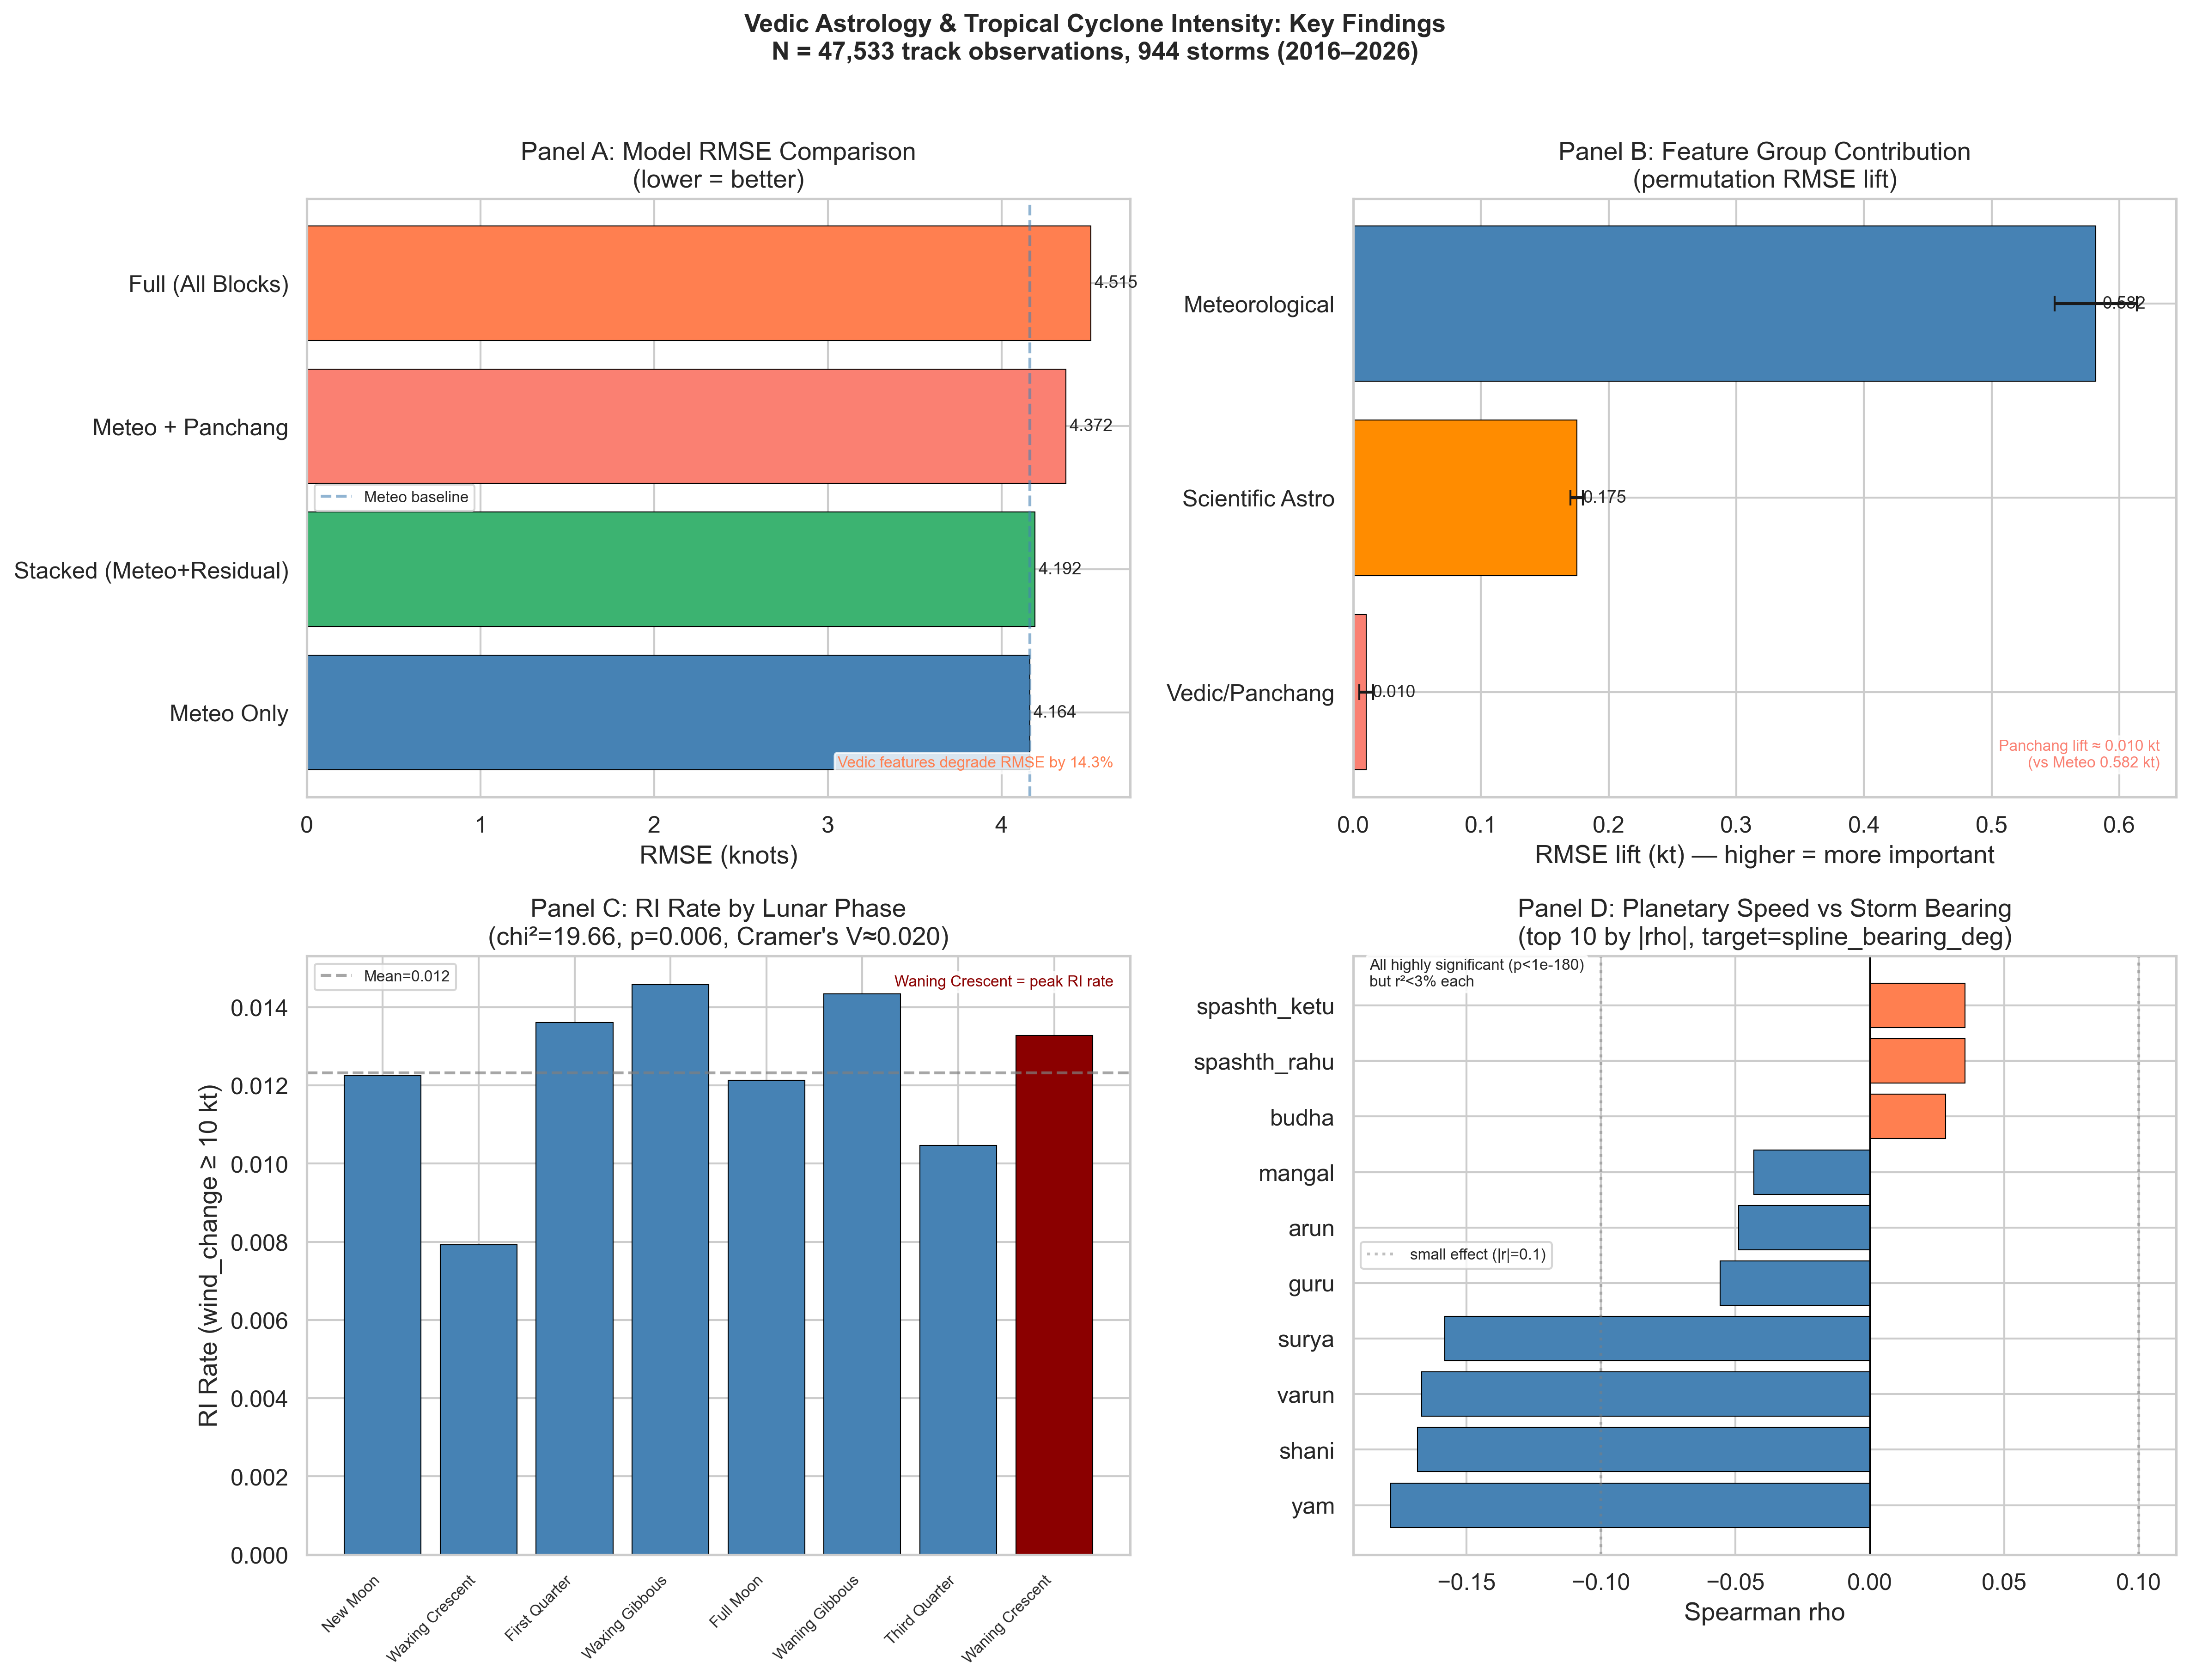
\includegraphics[width=\textwidth]{publication_figure.png}
  \caption{Four-panel publication figure.
           \textbf{(A)} Model RMSE comparison; the dashed blue line marks the
           meteorological baseline. Adding Vedic features monotonically increases
           error.
           \textbf{(B)} Feature group RMSE lift (permutation importance); the
           Vedic/Panchang lift of 0.010~kt is negligible.
           \textbf{(C)} RI rate by lunar phase; the Waning Crescent bar (dark red)
           is the peak phase, the dashed line marks the overall mean RI rate.
           \textbf{(D)} Top-10 Spearman $\rho$ between planetary speed and storm
           bearing; all values are negative (faster speed $\to$ more westward track)
           and all are statistically significant ($p < 10^{-20}$) but small
           ($r^2 < 0.032$).}
  \label{fig:pub}
\end{figure}

\end{document}
